\scanpage{85}
% archive foliation: 84
tel que la décomposition de $\unsure{\mathcal P|P}_n(X_1\times\cdots\times X_r;Y)$ en des $\unsure{\mathcal P|P}_{\nu_1,\ldots,\nu_r}(X_1,\ldots,X_r;Y)$ respecte les op. de $k$, i.e. $f\in \unsure{\mathcal P|P}_{\nu_1,\ldots,\nu_r}$ implique
\[f\circ(\mathrm{id}_{\lambda_1}\times\cdots\times\mathrm{id}_{\lambda_r})=\lambda_1^{\nu_1}\cdots\lambda_r^{\nu_r}f\]
pour tt $(\lambda_1,\ldots,\lambda_r)\in k^r$.
\figure{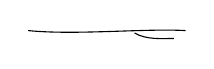
\begin{tikzpicture}\draw (0,0) .. controls (.6,-.06) and (1.5,.03) .. (2,0);\draw (1.35,-.03) .. controls (1.5,-.12) and (1.7,-.10) .. (1.85,-.10);\end{tikzpicture}}
\uline{Ex} La catégorie des $k$-modules est une $\otimes$-pd-catégorie.
De $\unsure{\Rightarrow}$ si $\unsure{\mathcal X|\mathcal T}$ un topos avec une $k$-Algèbre $K$, la cat. des $K$-Modules
\deleted{et \unsure{on p.}} [De $\unsure{\Rightarrow}$ on peut prendre des $K$-Modules gradués, \deleted{par un groupe} quelconque, \deleted{\unsure{compléter}} on \unsure{considère} des \unsure{pu. div.} $\Gamma^n(M^i)$ pour le degré $ni$.]
\margin{?}
\figure{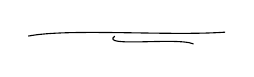
\begin{tikzpicture}\draw (0,0) .. controls (.5,.1) and (1.8,0) .. (2.5,.05);\draw (1.1,0) .. controls (.9,-.15) and (1.9,-.01) .. (2.1,-.1);\end{tikzpicture}}
Il y a diverses questions dans le cas ``abstrait''. Par exemple : quand et comment mettre sur $\Gamma^*(M)$ \inserted{($\forall M\in\operatorname{Ob}(\unsure{\mathcal P|P}_1)$)} une structure ``à p.d.'' ? i.e. des hom de degré $1$
\[\Gamma^p(\Gamma^q(M))\mathbin{-}\Gamma^{pq}(M)\]
satisfaisant aux axiomes des p.d. ?

